\documentclass[../main.tex]{subfiles}
\begin{document}
\chapter{2021-2022学年微积分（一）（下）期末考试}

\section{单项选择题(每小题 3 分，共 18 分)}
\begin{enumerate}
    \item 微分方程 \( y'' + y = x^2 + 1 + \sin x \) 的待定特解形式可设为（\qquad）.

          \begin{tasks}[label=\textbf{\Alph*.}, label-width=1.5em, column-sep=1em](2)
              \task \( y^* = ax^2 + bx + c + x(A\sin x + B\cos x) \)
              \task \( y^* = ax^2 + bx + c + A\sin x \)
              \task \( y^* = x(ax^2 + bx + c + A\sin x + B\cos x) \)
              \task \( y^* = ax^2 + bx + c + A\cos x \)
          \end{tasks}

    \item 在下列极限结果中，正确的是（\qquad）.

          \begin{tasks}[label=\textbf{\Alph*.}, label-width=1.5em, column-sep=1em](2)
              \task \( \lim\limits_{\substack{x \to 0 \\ y \to 0}} \dfrac{xy}{x^2 + y^2} = 0 \)
              \task \( \lim\limits_{\substack{x \to 0 \\ y \to 0}} \dfrac{x^2 y}{x^2 + y^2} = 0 \)
              \task \( \lim\limits_{\substack{x \to 0 \\ y \to 0}} \dfrac{xy}{x + y} = 0 \)
              \task \( \lim\limits_{\substack{x \to 0 \\ y \to 0}} \dfrac{x^2 y}{x + y} = 0 \)
          \end{tasks}

    \item 设 \( f(x) \) 为连续函数，\( F(t) = \displaystyle \int_1^t \mathrm{d}y \displaystyle \int_y^t f(x) \mathrm{d}x \)，则 \( F'(2) \) 等于（\qquad）.

          \begin{tasks}[label=\textbf{\Alph*.}, label-width=1.5em, column-sep=1em](2)
              \task \( 2f(2) \)
              \task \( f(2) \)
              \task \( -f(2) \)
              \task \( 0 \)
          \end{tasks}

    \item 设曲线 \( L: f(x, y) = 1 \)（\( f(x, y) \) 具有一阶连续偏导数），过第 II 象限内的点 \( M \) 和第 IV 象限内的点 \( N \)，\( T \) 为 \( L \) 上从点 \( M \) 到点 \( N \) 的一段弧，则下列积分小于零的是（\qquad）.

          \begin{tasks}[label=\textbf{\Alph*.}, label-width=1.5em, column-sep=1em](1)
              \task \( \displaystyle \int_T f(x, y) \mathrm{d}s \)
              \task \( \displaystyle \int_T f(x, y) \mathrm{d}x \)
              \task \( \displaystyle \int_T f(x, y) \mathrm{d}y \)
              \task \( \displaystyle \int_T f_x'(x, y) \mathrm{d}x + f_y'(x, y) \mathrm{d}y \)
          \end{tasks}

    \item 设 \( L \) 为空间曲线 \( \begin{cases} x^2 + y^2 + z^2 = a^2 \\ x + y + z = 0 \end{cases} \)，则 \( \displaystyle \oint_L x^2 \mathrm{d}s = \)（\qquad）.

          \begin{tasks}[label=\textbf{\Alph*.}, label-width=1.5em, column-sep=1em](2)
              \task \( 0 \)
              \task \( 2\pi a^3 \)
              \task \( \dfrac{1}{3}\pi a^2 \)
              \task \( \dfrac{2}{3}\pi a^3 \)
          \end{tasks}

    \item 设两个数列 \( \{a_n\}, \{b_n\} \)，若 \( \lim\limits_{n \to \infty} a_n = 0 \)，则（\qquad）.

          \begin{tasks}[label=\textbf{\Alph*.}, label-width=1.5em, column-sep=1em](1)
              \task 当 \( \sum \limits_{n=1}^{\infty} b_n \) 收敛时，\( \sum \limits_{n=1}^{\infty} a_n b_n \) 收敛
              \task 当 \( \sum \limits_{n=1}^{\infty} b_n \) 发散时，\( \sum \limits_{n=1}^{\infty} a_n b_n \) 发散
              \task 当 \( \sum \limits_{n=1}^{\infty} |b_n| \) 收敛时，\( \sum \limits_{n=1}^{\infty} a_n^2 b_n^2 \) 收敛
              \task 当 \( \sum \limits_{n=1}^{\infty} |b_n| \) 发散时，\( \sum \limits_{n=1}^{\infty} a_n^2 b_n^2 \) 发散
          \end{tasks}
\end{enumerate}

\section{填空题(每小题 4 分，共 16 分)}
\begin{enumerate}
    \setcounter{enumi}{6}
    \item 经过点 \( A(1,-2,3) \) 并且包含 \( x \) 轴的平面方程为 \(\underline{\hspace{5em}}\).
          \vspace{1em}

    \item 设向量场 \( \boldsymbol{A} = x^2 \boldsymbol{i} + y z \boldsymbol{j} + z x \boldsymbol{k} \)，则 \(  \text{rot}\boldsymbol{A} \Big|_{(1,1,2)} = \underline{\hspace{5em}}\).
          \vspace{1em}

    \item \( u = x e^{y}z^3 \) 在点 \( (1,1,1) \) 处的全微分 \( \mathrm{d}u = \underline{\hspace{5em}}\).
          \vspace{1em}

    \item 若将函数 \( f(x) = \pi - x \)（\( 0 \leq x \leq \pi \)）展开成正弦级数 \( \sum \limits_{n=1}^{\infty} b_n \sin nx \)，则系数 \( b_4 \) 的值为 \(\underline{\hspace{5em}}\).
          \vspace{1em}
\end{enumerate}

\section{基本计算题(每小题 7 分，共 42 分)}

\begin{enumerate}
    \setcounter{enumi}{10}
    \item 设方程组 \( \begin{cases} u + v = x, \\ u^2 + v^2 = y \end{cases} \) 确定隐函数 \( u = u(x,y), v = v(x,y) \)，且 \( u \neq v \)，求 \( \dfrac{\partial u}{\partial x} \)，\( \dfrac{\partial v}{\partial x} \).
          \vspace{15em}

    \item 设 \( \boldsymbol{n} \) 是曲面 \( S: z = x^2 + y^2 \) 在点 \( P_0(1,1,2) \) 处指向上侧的法向量，求函数 \( u = xz^3 - 3yz \) 在点 \( P_0 \) 处沿方向 \( \boldsymbol{n} \) 的方向导数 \( \dfrac{\partial u}{\partial \boldsymbol{n}} \).
          \vspace{9em}

    \item 计算 \( I = \displaystyle \iint \limits_D \max\{xy, 1\} \mathrm{d}x\,\mathrm{d}y \)，其中 \( D \) 是正方形区域 \( 0 \leq x \leq 2, 0 \leq y \leq 2 \).
          \vspace{9em}

    \item 计算 \( I = \displaystyle \iint \limits_{\Sigma} (xy + yz + zx) \mathrm{d}S \)，其中 \( \Sigma \) 为 \( z = \sqrt{x^2 + y^2} \) 被 \( x^2 + y^2 = 2ax \) 所截得的有限部分.
          \vspace{9em}

    \item 设 \( S \) 是球面 \( x^2 + y^2 + z^2 = R^2 \)（\( R > 0 \)）的外侧，求 \( I = \displaystyle \iint \limits_S x^3 \mathrm{d}y \mathrm{d}z + y^3 \mathrm{d}z \mathrm{d}x + z \mathrm{d}x \mathrm{d}y \).
          \vspace{9em}

    \item 确定幂级数 \( \sum \limits_{n=1}^{\infty} \dfrac{n}{n+1} x^n \) 的收敛域并求其和函数 \( S(x) \).
          \vspace{9em}
\end{enumerate}

\section{综合题(每小题 7 分，共 14 分)}
\begin{enumerate}
    \setcounter{enumi}{16}
    \item 若二阶常系数线性齐次微分方程 \( y'' + ay' + by = 0 \) 的通解为 \( y = (C_1 + C_2 x)\mathrm{e}^x \)，求非齐次方程 \( y'' + ay' + by = x \) 满足条件 \( y(0) = 2 \)，\( y'(0) = 0 \) 的解.
          \vspace{10em}

    \item 求 \( f(x, y) = x^2 + 2y^2 - x^2 y^2 \) 在区域 \( D = \{(x, y) \mid x^2 + y^2 \leq 4, y \geq 0\} \) 上的最大值和最小值.
          \vspace{10em}
\end{enumerate}

\section{证明题(每小题 5 分，共 10 分)}

\begin{enumerate}
    \setcounter{enumi}{18}
    \item 证明级数 \( \sum \limits_{n=1}^{\infty} \dfrac{(-1)^n}{n - (-1)^n} \) 是条件收敛的.
          \vspace{10em}

    \item 设函数 \( f(x) \) 在 \( (-\infty, +\infty) \) 内具有一阶连续导数，\( L \) 是上半平面 \( (y > 0) \) 内的有向分段光滑曲线，其始点为 \( (a, b) \)，终点为 \( (c, d) \).记 \( I = \displaystyle \int_L \dfrac{1}{y}[1 + y^2 f(xy)]\mathrm{d}x + \dfrac{x}{y^2}[y^2 f(xy) - 1]\mathrm{d}y \)，(1) 证明曲线积分 \( I \) 与路径 \( L \) 无关；(2) 当 \( ab = cd \) 时，求 \( I \) 的值.
          \vspace{10em}
\end{enumerate}
\chapter{2021-2022学年微积分（一）（下）期末考试参考答案}
\section{单项选择题(每小题 3 分，共 18 分)}
\begin{enumerate}
    \item \textbf{Solution}. A.

          方程对应的齐次方程 \( y'' + y = 0 \) 的特征方程 \( r^2 + 1 = 0 \) 有两个单根 \( r = i, -i \)，所以齐次方程的通解为
          \[
              y = C_1 \cos x + C_2 \sin x.
          \]
          对于非齐次项$x^2+1$，特解可以设为$y_1=ax^2+bx+c$；

          对于非齐次项$\sin x$，由于$\lambda=i$是特征方程的根，所以特解可以设为$y_2=x(A\sin x+B\cos x)$，

          由解的叠加原理，非齐次方程的特解可以设为
          \[
              y^* = ax^2 + bx + c + x(A\sin x + B\cos x).
          \]

    \item \textbf{Solution}. B.

          对于A选项，当$(x,y)\to(0,0)$且$y=x$时，$\lim\limits_{x\to0}\frac{x^2}{2x^2}=\frac{1}{2}$；

          当$(x,y)\to(0,0)$且$y=-x$时，$\lim\limits_{x\to0}\frac{-x^2}{2x^2}=-\frac{1}{2}$，所以A选项错误；

          对于B选项，因为
          \[
              \left|\frac{x^2 y}{x^2+y^2}\right|\leq |y|,
          \]
          所以由夹逼准则可知$\lim\limits_{(x,y)\to(0,0)}\frac{x^2 y}{x^2+y^2}=0$，所以B选项正确；

          对于C选项，当$(x,y)\to(0,0)$且$y=x^2-x$时，$\lim\limits_{x\to0}\frac{x\left(x^2-x\right)}{x^2}=-1$；

          当$(x,y)\to(0,0)$且$y=x$时，$\lim\limits_{x\to0}\frac{x^2}{2x}=0$，所以C选项错误；

          对于D选项，当$(x,y)\to(0,0)$且$y=x^3-x$时，$\lim\limits_{x\to0}\frac{x^2\left(x^3-x\right)}{x^3}=-1$；

          当$(x,y)\to(0,0)$且$y=x$时，$\lim\limits_{x\to0}\frac{x^3}{2x}=0$，所以D选项错误.

    \item \textbf{Solution}. B.

          先交换积分顺序
          \[
              F(t)=\int_1^t\,\mathrm{d}y\int_y^t f(x)\,\mathrm{d}x=\int_{1}^{t}\,\mathrm{d}x\int_{1}^{x}f(x)\,\mathrm{d}y=\int_1^t(x-1)f(x)\,\mathrm{d}x.
          \]
          因而
          \[
              F'(t)=(t-1)f(t),
          \]
          所以
          \[
              F'(2)=f(2).
          \]

    \item \textbf{Solution}. C.

          因为在曲线 \(L:f(x,y)=1\) 上恒有 \(f(x,y)=1\)，故
          \[
              \int_T f(x,y)\,\mathrm{d}y=\int_T \mathrm{d}y=y_N-y_M<0,
          \]
          其中因 \(M\) 在第二象限、\(N\) 在第四象限，所以 \(y_N<y_M\).

    \item \textbf{Solution}. D.

          交线 \(L\) 是球面与过原点平面相交得到的大圆，因此半径为 \(a\). 由对称性可知
          \[
              \oint_L x^2\,\mathrm{d}s=\oint_L y^2\,\mathrm{d}s=\oint_L z^2\,\mathrm{d}s.
          \]
          又
          \[
              \oint_L(x^2+y^2+z^2)\,\mathrm{d}s=a^2\oint_L\,\mathrm{d}s=a^2\cdot 2\pi a=2\pi a^3.
          \]
          三者相等，所以
          \[
              \oint_L x^2\,\mathrm{d}s=\frac{2\pi a^3}{3}.
          \]

    \item \textbf{Solution}. C.

          对于A选项，令$a_n=b_n=\frac{(-1)^n}{\sqrt{n}}$，则$\lim\limits_{n\to\infty}a_n=0$，且$\sum_{n=1}^{\infty}b_n$收敛，

          但$\sum_{n=1}^{\infty}a_n b_n=\sum_{n=1}^{\infty}\frac{1}{n}$发散，所以A选项错误；

          对于B选项，令$a_n=b_n=\frac{1}{n}$，则$\lim\limits_{n\to\infty}a_n=0$，且$\sum_{n=1}^{\infty}b_n$发散，

          但$\sum_{n=1}^{\infty}a_n b_n=\sum_{n=1}^{\infty}\frac{1}{n^2}$收敛，所以B选项错误；

          对于C选项，由于$\lim_{n\to\infty}a_n=0$，则对于充分大的$N_1$，当$n>N_1$时，有$|a_n|<1$；

          且$\sum_{n=1}^\infty |b_n|$收敛，根据级数收敛的必要条件可知 $\lim_{n\to\infty} |b_n| = 0$，

          于是同理存在充分大的$N_2$，当$n>N_2$时，有$|b_n|<1$，所以当$n>\max\{N_1,N_2\}$时，$a_n^2 b_n^2 \leq b_n^2\leq |b_n|$，

          由比较判别法可知$\sum_{n=1}^\infty a_n^2 b_n^2$收敛，所以C选项正确；

          对于D选项，令$a_n=\frac{1}{n}$，$b_n=1$，则$\lim\limits_{n\to\infty}a_n=0$，且$\sum_{n=1}^{\infty} |b_n|$发散，

          但$\sum_{n=1}^{\infty} a_n^2 b_n^2=\sum_{n=1}^{\infty} \frac{1}{n^2}$收敛，所以D选项错误.
\end{enumerate}

\section{填空题(每小题 4 分，共 16 分)}
\begin{enumerate}
    \setcounter{enumi}{6}
    \item \textbf{Solution}. $3y+2z=0$.

          由于所求平面包含 \(x\) 轴，所以它含有方向向量 \((1,0,0)\). 又它经过点 \(A(1,-2,3)\)，故还含有向量 \((1,-2,3)\).

          两向量叉积可取法向量
          \[
              (1,0,0)\times(1,-2,3)=(0,-3,-2),
          \]
          所以平面方程为
          \[
              3y+2z=0.
          \]

    \item \textbf{Solution}. $-\boldsymbol{i}-2\boldsymbol{j}$.

          \[
              \boldsymbol{A}=(x^2,yz,zx),
          \]
          因而
          \[
              \begin{aligned}
                  \operatorname{rot}\boldsymbol{A}= {} & \begin{vmatrix}
                                                          \boldsymbol{i}              & \boldsymbol{j}              & \boldsymbol{k}              \\
                                                          \frac{\partial}{\partial x} & \frac{\partial}{\partial y} & \frac{\partial}{\partial z} \\
                                                          x^2                         & yz                          & zx
                                                      \end{vmatrix}
                  =                                  \left(\frac{\partial(zx)}{\partial y}-\frac{\partial(yz)}{\partial z},
                  \frac{\partial(x^2)}{\partial z}-\frac{\partial(zx)}{\partial x},
                  \frac{\partial(yz)}{\partial x}-\frac{\partial(x^2)}{\partial y}\right)                                                         \\
                  = {} & (-y,-z,0).
              \end{aligned}
          \]
          在 \((1,1,2)\) 处取值即得
          \[
              -\boldsymbol{i}-2\boldsymbol{j}.
          \]

    \item \textbf{Solution}. $\mathrm{e}\,\mathrm{d}x+\mathrm{e}\,\mathrm{d}y+3\mathrm{e}\,\mathrm{d}z$.

          \[
              u=x\mathrm{e}^yz^3,\quad u_x=\mathrm{e}^yz^3,\quad u_y=x\mathrm{e}^yz^3,\quad u_z=3x\mathrm{e}^yz^2.
          \]
          在 \((1,1,1)\) 处有 \(u_x=u_y=\mathrm{e},\ u_z=3\mathrm{e}\)，故
          \[
              \mathrm{d}u=\mathrm{e}\,\mathrm{d}x+\mathrm{e}\,\mathrm{d}y+3\mathrm{e}\,\mathrm{d}z.
          \]

    \item \textbf{Solution}. $\dfrac12$.

          由
          \[
              b_n=\frac{2}{\pi}\int_0^\pi(\pi-x)\sin nx\,\mathrm{d}x,
          \]
          当 \(n=4\) 时
          \[
              \begin{aligned}
                  b_4 & = \frac{2}{\pi}\int_0^\pi(\pi-x)\sin 4x\,\mathrm{d}x                                         \\
                      & = \frac{2}{\pi}\int_{0}^{\pi}x\sin 4(\pi-x)\,\mathrm{d}x                                     \\
                      & = -\frac{2}{\pi}\int_{0}^{\pi}x\sin 4x\,\mathrm{d}x                                          \\
                      & = \frac{1}{2\pi}\left[x\cos 4x\Big|_0^\pi-\int_0^\pi\cos 4x\,\mathrm{d}x\right]=\frac{1}{2}. \\
              \end{aligned}
          \]
\end{enumerate}

\section{基本计算题(每小题 7 分，共 42 分)}
\begin{enumerate}
    \setcounter{enumi}{10}
    \item \textbf{Solution}. 对方程组$\begin{cases}
                  u+v=x, \\
                  u^2+v^2=y
              \end{cases}$
          关于 \(x\) 求偏导，得
          \[
              \begin{cases}
                  u_x+v_x=1, \\
                  2uu_x+2vv_x=0.
              \end{cases}
          \]
          解得
          \[
              u_x=\frac{v}{v-u},\qquad v_x=-\frac{u}{v-u}.
          \]

    \item \textbf{Solution}. 曲面写成
          \[
              z-x^2-y^2=0,
          \]
          所以上侧法向量可取
          \[
              \boldsymbol{n}=(-2x,-2y,1).
          \]
          在 \(P_0(1,1,2)\) 处，
          \[
              \boldsymbol{n}=(-2,-2,1),\qquad \boldsymbol{n}_0=\frac13(-2,-2,1).
          \]
          又
          \[
              u=xz^3-3yz,\qquad \nabla u=(z^3,-3z,3xz^2-3y),
          \]
          所以
          \[
              \nabla u(P_0)=(8,-6,9).
          \]
          因而方向导数为
          \[
              \frac{\partial u}{\partial \boldsymbol{n}}\Big|_{P_0}
              =\nabla u(P_0)\cdot \boldsymbol{n}_0
              =\frac{-16+12+9}{3}
              =\frac53.
          \]

    \item \textbf{Solution}. 如图，按曲线 \(xy=1\) 将区域$D$分为$D_1=\{(x,y)\in D\mid xy\ge 1\}$和$D_2=\{(x,y)\in D\mid xy<1\}$.

          \noindent
          \begin{minipage}[c]{0.58\textwidth}
              当 \(xy<1\) 时 \(\max\{xy,1\}=1\)，当 \(xy\ge 1\) 时 \(\max\{xy,1\}=xy\). 故
              \[
                  I=\iint\limits_{D_1}xy\,\mathrm{d}x\,\mathrm{d}y
                  +\iint\limits_{D_2}\,\mathrm{d}x\,\mathrm{d}y.
              \]
              逐段积分得
              \[
                  \begin{aligned}
                      I= {} & \int_{\frac{1}{2}}^2x\,\mathrm{d}x\int_{\frac{1}{x}}^2y\,\mathrm{d}y
                      +\int_0^{\frac{1}{2}}\,\mathrm{d}y\int_0^2\,\mathrm{d}x
                      +\int_{\frac{1}{2}}^2\,\mathrm{d}x\int_0^{\frac{1}{x}}\,\mathrm{d}y       \\
                      = {} & \frac{19}{4}+\ln2.
                  \end{aligned}
              \]
          \end{minipage}
          \hfill %
          \begin{minipage}[c]{0.38\textwidth}
              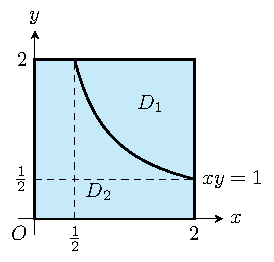
\includegraphics[width=4.6cm]{2022xf-figure1.pdf} % 引入图片源
          \end{minipage}

    \item \textbf{Solution}. 曲面 \(\Sigma:z=\sqrt{x^2+y^2}\) 关于 \(xOz\) 面对称，而 \(xy\) 与 \(yz\) 都关于 \(y\) 为奇函数，因此
          \[
              \iint\limits_\Sigma xy\,\mathrm{d}S=\iint\limits_\Sigma yz\,\mathrm{d}S=0.
          \]
          从而
          \[
              I=\iint\limits_\Sigma zx\,\mathrm{d}S.
          \]
          投影到 \(xOy\) 面，因
          \[
              z_x=\frac{x}{\sqrt{x^2+y^2}},\qquad z_y=\frac{y}{\sqrt{x^2+y^2}},
          \]
          所以
          \[
              \mathrm{d}S=\sqrt{1+z_x^2+z_y^2}\,\mathrm{d}x\,\mathrm{d}y=\sqrt2\,\mathrm{d}x\,\mathrm{d}y.
          \]
          用极坐标 \(x=r\cos\theta,\ y=r\sin\theta\)，区域为
          \[
              -\frac{\pi}{2}\le \theta\le \frac{\pi}{2},\quad 0\le r\le 2a\cos\theta.
          \]
          又 \(z=r\)，故
          \[
              \begin{aligned}
                  I= {} & \sqrt2\int_{-\frac{\pi}{2}}^{\frac{\pi}{2}}\,\mathrm{d}\theta\int_0^{2a\cos\theta} r^3\cos\theta\,\mathrm{d}r                                      \\
                  = {} & 4\sqrt2 a^4\int_{-\frac{\pi}{2}}^{\frac{\pi}{2}}\cos^5\theta\,\mathrm{d}\theta = 8\sqrt{2} a^4\int_0^{\frac{\pi}{2}}\cos^5\theta\,\mathrm{d}\theta \\
                  = {} & 8\sqrt{2} a^4\cdot \frac{4}{5}\cdot\frac{2}{3} = \frac{64\sqrt2}{15}a^4.
              \end{aligned}
          \]

    \item \textbf{Solution}. 由Gauss公式可得
          \[
              I=\iiint\limits_V\left(\frac{\partial x^3}{\partial x}+\frac{\partial y^3}{\partial y}+\frac{\partial z}{\partial z}\right)\,\mathrm{d}v
              =\iiint\limits_V(3x^2+3y^2+1)\,\mathrm{d}v.
          \]
          再利用球域的轮换对称性，
          \[
              \iiint\limits_V(3x^2+3y^2)\,\mathrm{d}v=2\iiint\limits_V(x^2+y^2+z^2)\,\mathrm{d}v.
          \]
          因而
          \[
              \begin{aligned}
                  I= {} & 2\int_{0}^{2\pi}\,\mathrm{d}\theta\int_{0}^{\pi}\sin\varphi\,\mathrm{d}\varphi\int_{0}^{R}r^4\,\mathrm{d}r+\frac{4}{3}\pi R^3 \\
                  = {} & \frac{8\pi R^5}{5}+\frac{4\pi R^3}{3}.
              \end{aligned}
          \]

    \item \textbf{Solution}. 用比值判别法，令$a_n=\frac{n}{n+1}$，则
          \[
              \lim_{n\to\infty}\left|\frac{a_{n+1}}{a_n}\right|=\lim_{n\to\infty}\left|\frac{(n+1)}{(n+2)}\cdot\frac{n+1}{n}\right|=1,
          \]
          因此级数的收敛半径为$1$. 当$x=1$时，$\lim_{n\to\infty}\frac{n}{n+1}\neq0$，所以级数发散；

          当$x=-1$时，$\lim_{n\to\infty}\frac{n}{n+1}(-1)^n$不存在，所以级数发散. 故级数的收敛域为$(-1,1)$.

          当$x=0$时，$S(0)=0$. 当$-1<x<1$时，
          \[
              \begin{aligned}
                  \sum_{n=1}^{\infty}\frac{n}{n+1}x^n = {} & \sum_{n=1}^{\infty}\left(1-\frac{1}{n+1}\right)x^n = \sum_{n=1}^{\infty}x^n - \sum_{n=1}^{\infty}\frac{x^n}{n+1} \\
                  = {} & \frac{x}{1-x} - \frac{1}{x}\sum_{n=1}^{\infty}\int_{0}^{x}t^n\,\mathrm{d}t                                       \\
                  = {} & \frac{x}{1-x} - \frac{1}{x}\int_{0}^{x}\frac{t}{1-t}\,\mathrm{d}t                                                \\
                  = {} & \frac{x}{1-x} - \frac{1}{x}\left[-x-\ln(1-x)\right] = \frac{x}{1-x} + 1 + \frac{\ln(1-x)}{x}.
              \end{aligned}
          \]

          综上所述，$S(x)=\begin{cases}
                  0,                                      & x=0,    \\
                  \frac{x}{1-x} + 1 + \frac{\ln(1-x)}{x}, & -1<x<1.
              \end{cases}$
\end{enumerate}

\section{综合题(每小题 7 分，共 14 分)}
\begin{enumerate}
    \setcounter{enumi}{16}
    \item \textbf{Solution}. 由齐次方程通解
          \[
              y=(C_1+C_2x)\mathrm{e}^x
          \]
          可知特征方程有二重根 \(r=1\)，于是
          \[
              y''-2y'+y=0.
          \]
          因而原非齐次方程为
          \[
              y''-2y'+y=x.
          \]
          设特解为 \(y^*=Ax+B\)，代入得
          \[
              Ax+B-2A=x,
          \]
          比较系数得 \(A=1,\ B=2\). 所以通解为
          \[
              y=(C_1+C_2x)\mathrm{e}^x+x+2.
          \]
          由条件
          \[
              y(0)=2,\qquad y'(0)=0
          \]
          解得 \(C_1=0,\ C_2=-1\). 因而
          \[
              y=-x\mathrm{e}^x+x+2.
          \]

    \item \textbf{Solution}. 在区域内部，令
          \[
              \begin{cases}
                  f_x=2x(1-y^2)=0, \\
                  f_y=2y(2-x^2)=0,
              \end{cases}
          \]
          解得驻点为 \((0,0),(\pm\sqrt2,1)\)，其函数值分别为
          \[
              f(0,0)=0,\qquad f(\pm\sqrt2,1)=2.
          \]
          边界分两部分考察. 当 \(y=0\) 时，$f(x,0)=x^2$，$-2\le x\le 2$，所以最小值为 \(0\)，最大值为 \(4\).

          当 \(x^2+y^2=4 \) 时，代入 \(y^2=4-x^2\) 得$f=x^4-5x^2+8=\left(x^2-\frac{5}{2}\right)^2+\frac{7}{4}$，$-2\le x\le 2$，

          所以最小值为 \(\frac{7}{4}\)，最大值为 \(8\).

          比较边界与内部函数值，得全区域上
          \[
              \max f=8,\qquad \min f=0.
          \]
\end{enumerate}

\section{证明题(每小题 5 分，共 10 分)}
\begin{enumerate}
    \setcounter{enumi}{18}
    \item \textbf{Proof}. 设
          \[
              a_n=\frac{(-1)^n}{n-(-1)^n}.
          \]
          先看绝对收敛性. 注意到
          \[
              |a_n|=\frac{1}{n-(-1)^n}\sim \frac{1}{n}\qquad (n\to\infty),
          \]
          故 \(\sum_{n=1}^{\infty} |a_n|\) 发散. 当$n\geq2$时，设
          \[
              a_n=\frac{(-1)^n\left(n+(-1)^n\right)}{\left(n-(-1)^n\right)\left(n+(-1)^n\right)}=(-1)^n\frac{n}{n^2-1}+\frac{1}{n^2-1}=u_n+v_n,
          \]
          其中 $u_n=(-1)^n\frac{n}{n^2-1}$ 由Leibniz判别法可知收敛，$v_n=\frac{1}{n^2-1}\sim \frac{1}{n^2}$ 也收敛.

          所以$\sum_{n=1}^{\infty} a_n$ 条件收敛.

    \item \textbf{Proof}. 记
          \[
              P(x,y)=\frac{1}{y}[1+y^2f(xy)],\qquad
              Q(x,y)=\frac{x}{y^2}[y^2f(xy)-1].
          \]
          直接计算得
          \[
              P_y=f(xy)-\frac{1}{y^2}+xyf'(xy),\qquad
              Q_x=f(xy)-\frac{1}{y^2}+xyf'(xy),
          \]
          即 \(P_y=Q_x\). 因而在上半平面 \(y>0\) 内该积分与路径无关.

          下面求势函数$\Phi(x,y)$. 设$F'(t)=f(t)$，由
          \[
              \Phi_x=P(x,y)=\frac{1}{y}+yf(xy)
          \]
          对$x$积分，得
          \[
              \Phi(x,y)=\int\left(\frac{1}{y}+yf(xy)\right)\mathrm{d}x
              =\frac{x}{y}+F(xy)+\varphi(y),
          \]
          其中 \(\varphi(y)\) 只与 \(y\) 有关. 再对 \(y\) 求偏导，
          \[
              \Phi_y=-\frac{x}{y^2}+xf(xy)+\varphi'(y).
          \]
          与
          \[
              Q(x,y)=xf(xy)-\frac{x}{y^2}
          \]
          比较可得 \(\varphi'(y)=0\)，故可取
          \[
              \Phi(x,y)=\frac{x}{y}+F(xy).
          \]
          因而
          \[
              I=\Phi(c,d)-\Phi(a,b)=\frac{c}{d}-\frac{a}{b}+F(cd)-F(ab).
          \]
          当 \(ab=cd\) 时，最后两项相消，所以
          \[
              I=\frac{c}{d}-\frac{a}{b}.
          \]
\end{enumerate}
\end{document}






